\documentclass[12pt, letterpaper]{article}
\usepackage[utf8]{inputenc}
\usepackage[spanish]{babel}
\usepackage{hyperref}
\usepackage{multicol}
\usepackage{graphicx}
\usepackage{float}
\graphicspath{{images/}}

\title{Traducción automática}
\author{Mateo Gonzalez Ocampo \and Juan Alejandro Uribe Ramirez}
\date{Junio 2020}

\begin{document}
    \maketitle
    \begin{abstract}
        En el siguiente trabajo se realiza una revisión de algunos de los métodos que se han usado históricamente para resolver el problema de la 
        traducción automática. Los métodos seleccionados fueron la traducción basada en reglas, basada en ejemplos y basada en redes neuronales.
        Para cada método se presenta una pequeña introducción histórica, un análisis de como funciona y aplicaciones destacadas. Finalmente se presentan 
        algunas conclusiones acerca de lo encontrado en la literatura durante la investigación de estos métodos.

    \end{abstract}
    \begin{multicols}{2}
        \section{Introducción}
            La traducción automática se refiere al uso de computadores para realizar traducciones
            de un lenguaje SL (\textit{Source Language}) a un lenguaje TL (\textit{Target Language}).
        \section{Métodos}
            \subsection{Reglas}
                Los sistemas basados en reglas constituyen los primeros intentos usados para la creación
                de traductores automáticos y fueron ampliamente usados entre la decada de las 60 y la 
                primera parte de los 80. Estos sistemas usan un conjunto de reglas escritas a mano para la
                transformación de SL a TL, ademas de un diccionario para la traducción de palabras. 

                \begin{figure}[H]
                    \centering
                    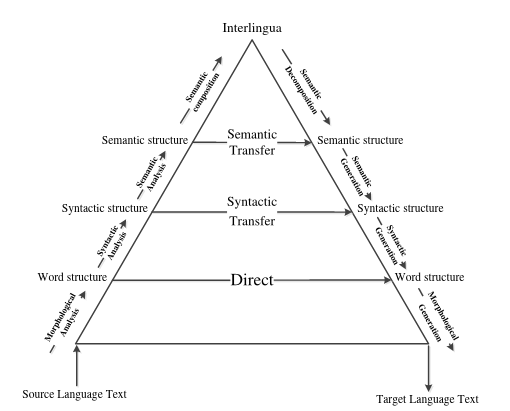
\includegraphics[width=0.4\textwidth]{triangle.png}
                    \caption[]{Triangulo de Vauquois.}
                    \label{triangle}
                \end{figure}
                
                
                Se pueden diferenciar los métodos usados en este tipo de sistemas en dos generaciones\cite{HUTCHINS1995431}:
                La primera, se caracteriza porque la transformación de SL a TL es directa, es decir, se traduce
                cada palabra por separado, usando un diccionario de SL a TL, y al resultado de esta transformación
                se le aplican un conjunto de reglas para hacer que la nueva oración sea coherente en TL, lo que 
                puede involucrar una reorganización de las palabras del texto generado. A este tipo de métodos se 
                les conoce como métodos de traducción directa.

                La segunda generación de métodos, conocidos como de traducción indirecta, transforman inicialmente el texto
                en SL a una representación intermedia a partir de la cual se transforma a TL. Existen varios modelos para
                la generación de dicha representación, siendo los mas conocidos los métodos de interlingua y de transferencia 
                \cite{Musatafa}\cite{HUTCHINS1995431}\cite{Mohamed}. En el primero se asume que la representación intermedia es 
                unica para todos los lenguajes, por lo que solo es necesario definir reglas para transformar a este estado 
                intermedio y desde este estado intermedio. Esto, basado en las ideas planteadas por Descartes en el siglo XVII 
                acerca de la existencia de un lenguaje universal. En el segundo método cada lenguaje tiene su propia representación 
                intermedía, lo que implica que ademas de las reglas relacionadas con la representación intermedia, es necesario un 
                conjunto de reglas adicional para transformar de una representación a otra. En la figura \ref{triangle} se muestra el 
                triangulo de Vauquois, el cual sirve para entender los diferentes niveles de análisis entre los métodos mencionados 
                anteriormente. 
                
                
                \href{https://www.systransoft.com/} {SYSTRAN}, \href{https://www.apertium.org}{APERTIUM} y \href{https://gramtrans.com}{GramTrans}
                son algunos ejemplos de aplicaciones que usan sistemas basados en reglas.
                
                
            \subsection{Ejemplos}
                Los sistemas basados en ejemplos surgieron durante la decada de los 80, debido principalmente al trabajo de Nagao\cite{Nagao}, el cual planteaba
                una nueva forma de traducción automática basada en la idea de que el ser humano no traduce partiendo de análisis lingüísticos complejos, sino
                descomponiendo el texto a traducir en fragmentos los cuales son luego traducidos y reorganizados para formar el nuevo texto. De manera similar 
                a los sistemas basados en reglas, los sistemas basados en ejemplos hacen uso de un diccionario de SL a TL junto con una base de datos de ejemplos, 
                la cual se usa para como base para la traducción (En contraste con las reglas usadas en los sistemas basados en reglas). También suele usarse un 
                Tesauro como parte de la base de datos. Un ejemplo esta constituido por dos textos en dos lenguajes, siendo ambos textos traducciones de si mismos\cite{Haihua}.
                
                Existen tres etapas en el proceso de traducción mediante ejemplos \cite{Nagao}\cite{Sumita2005TranslatingWE}:
                \begin{enumerate}
                    \item Como primer paso, se realiza un análisis del texto, para identificar los fragmentos que mejor se relacionen con los textos de la base de
                    datos.
                    \item Luego, usando los fragmentos obtenidos, se extraen de la base de datos los ejemplos que mas se asemejen a los fragmentos. Los ejemplos se
                    seleccionan con base en alguna métrica que toma ambos textos y asigna un grado de similaridad entre ellos.  
                    \item Finalmente, con base en los ejemplos obtenidos de la base de datos, se genera el texto traducido.
                \end{enumerate}

                \begin{figure}[H]
                    \centering
                    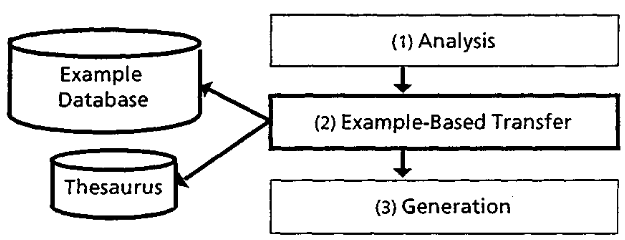
\includegraphics[width=0.4\textwidth]{example.png}
                    \caption[]{Configuración de un sistema basado en ejemplos Tomado de \cite{Sumita2005TranslatingWE}.}
                    \label{example}
                \end{figure}
                 
                Los sistemas basados en ejemplos resuelven algunos de los problemas presentes en los sistemas basados en reglas\cite{Sumita2005TranslatingWE}, principalmente
                la dificultad y complejidad de añadir nuevas reglas a un sistema ya establecido, dado que pueden haber conflictos con las reglas previamente establecidas. 
                \href{http://cunei.sourceforge.net/}{Cunei} y \href{http://www.cs.cmu.edu/~ralf/ebmt/ebmt.html}{CMU-EBMT} son probablemente de los sistemas basados en ejemplos
                mas reconocidos.
            \subsection{Redes neuronales}
                Los fundamentos matematicos de las redes neuronales...

            \bibliographystyle{unsrt}
            \bibliography{references}
    \end{multicols}
    
\end{document} 
